\documentclass[a4paper,12pt]{scrreprt}

\usepackage[italian]{babel}

\usepackage[utf8]{inputenc}

\usepackage{graphicx}
\graphicspath{{images/}}

\usepackage{tcolorbox}
\tcbuselibrary{theorems,minted}
\newtcbtheorem[number within=chapter]{mynote}{Nota}{%
  colback=blue!5,
  colframe=blue!35!black,
  fonttitle=\bfseries,
  before={\vspace{0.5cm}},
  after={\vspace{0.5cm}}}{note}
\newtcblisting{myvhdl}[1]{%
  listing only,
  minted language=vhdl,
  minted options=breaklines,
  fonttitle=\bfseries,
  title=#1
}
\newcommand{\BashFancyFormatLine}{%
  \def\FancyVerbFormatLine##1{\$\,##1}%
}
\newtcblisting{commandshell}{%
  colback=black,
  colupper=white,
  colframe=yellow!75!black,
  listing only,
  minted options={formatcom=\BashFancyFormatLine},
  minted language=bash}

\usepackage{hyperref}

\usepackage{courier}
\usepackage{listings}
\lstset{
  basicstyle=\ttfamily,
}

\title{Il Processore Mic-1 \\
  \ \\
  \large Dispensa didattica del corso di\\
  Architettura dei Sistemi di Elaborazione}
\author{Prof.\ Nicola Mazzocca \\
  Ing.\ Alberto Moriconi}
\date{}

\begin{document}
\maketitle

\chapter{Il Livello Microarchitetturale}

Il processore Mic-1 è un utile esempio didattico, presentato in~\cite{tanenbaum}
per due scopi principali:
\begin{enumerate}
  \item mostrare come, usando elementi logici di base come quelli già studiati
  nel corso, sia possibile realizzare una microarchitettura che implementi un
  semplice set di istruzioni;
  \item mostrare come anche la realizzazione di un sistema apparentemente
  complesso come un processore si riduca in realtà alla progettazione di
  un'unità operativa e di un'unità di controllo, e del modo in cui devono
  comunicare.
\end{enumerate}

In particolare, il set di istruzioni implementato dal Mic-1 è un sottoinsieme di
quello della Java Virtual Machine, denominato \textbf{IJVM} in quanto opera
unicamente sugli interi.

Una particolarità di questo processore è quella di non disporre di registri
generali; la sua architettura è infatti detta \textit{a stack}, in quanto le sue
istruzioni aritmetiche e logiche non hanno operandi espliciti, ma li prelevano
da una struttura \textit{last-in-first-out} allocata nella memoria principale,
su cui devono essere posti in precedenza.

\medskip

Consideriamo ad esempio l'esecuzione dell'operazione di somma e assegnazione

\begin{tcblisting}{listing only}
  a1 = a2 + a3
\end{tcblisting}

che è tradotta in linguaggio assembly IJVM come

\begin{tcblisting}{listing only}
  ILOAD a2
  ILOAD a3
  IADD
  ISTORE a1
\end{tcblisting}

Lo stato dello stack durante l'esecuzione evolve come in
fig.~\ref{fig:stack_add}; inizialmente, le locazioni di memoria \lstinline{a2} e
\lstinline{a3} contengono gli operandi, mentre la locazione \lstinline{a1} è non
inizializzata; dunque
\renewcommand{\labelenumi}{(\alph{enumi})}
\begin{enumerate}
  \item la prima istruzione \lstinline{ILOAD} legge il contenuto della locazione
  di memoria \lstinline{a2} e ne esegue il push su stack;
  \item la seconda istruzione \lstinline{ILOAD} legge il contenuto della
  locazione di memoria \lstinline{a3} e ne esegue il push su stack;
  \item l'istruzione \lstinline{IADD} esegue il pop dei due elementi in cima
  allo stack e il push della loro somma;
  \item l'istruzione \lstinline{ISTORE} esegue il pop della somma e lo scrive in
  memoria alla locazione \lstinline{a1}.
\end{enumerate}
\renewcommand{\labelenumi}{\arabic{enumi}.}

\begin{figure}
  \centering
  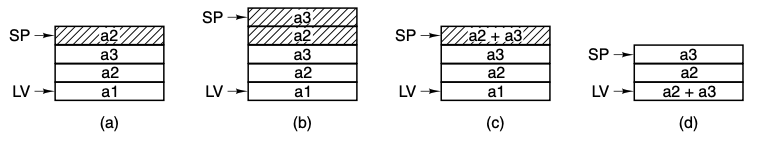
\includegraphics[width=\textwidth]{stack_add.png}
  \caption{Evoluzione dello stack durante le operazioni di somma e
    assegnazione}\label{fig:stack_add}
\end{figure}

Supponiamo che il processore si trovi al passo (c) e debba eseguire l'operazione
\lstinline{IADD}; per farlo deve, in prima analisi:
\begin{enumerate}
  \item eseguire un primo accesso in memoria, per prelevare il primo operando;
  \item eseguire un secondo accesso in memoria, per prelevare il secondo
  operando;
  \item sommare i due operandi;
  \item eseguire un terzo accesso in memoria, per scrivere il risultato.
\end{enumerate}

Per capire come è effettivamente possibile implementare queste operazioni, è
necessario introdurre l'unità operativa del processore.

\section{L'Unità Operativa}
L'unità operativa del processore che intendiamo progettare comprende l'ALU, i
suoi ingressi e le sue uscite (tra cui i registri che si interfacciano con la
memoria), ed è mostrata in fig.~\ref{fig:datapath}.

\begin{figure}
  \centering
  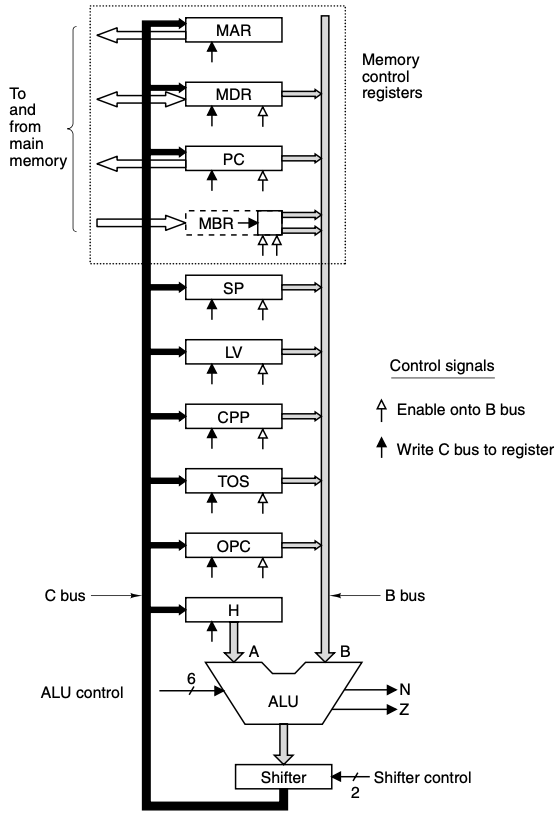
\includegraphics[width=0.9\textwidth]{datapath.png}
  \caption{Parte operativa del processore Mic-1}\label{fig:datapath}
\end{figure}

I registri hanno dimensione di 32 bit e non sono accessibili al programmatore,
ma solo al microprogramma.

\begin{mynote}{}{}
  Quando diciamo che i registri non sono accessibili al programmatore intendiamo
  che essi non fanno parte del \textit{modello di programmazione}, i.e.~non
  vengono utilizzati esplicitamente come operandi delle istruzioni. Vengono
  invece utilizzati dal microprogramma per implementare le istruzioni stesse.
\end{mynote}

L'unità operativa dispone di due bus, indicati con \lstinline{B} e
\lstinline{C}, collegati rispettivamente al secondo ingresso e all'uscita
dell'ALU; il primo ingresso dell'ALU è invece collegato esclusivamente al
registro \lstinline{H}.

Quasi tutti

\subsection{L'Unità Aritmetico Logica}

L'ALU è controllata mediante sei linee di controllo, che consideriamo asserite
se poste a $1$:
\begin{itemize}
  \item \lstinline{F0} e \lstinline{F1} determinano l'operazione da eseguire,
  \item \lstinline{ENA} e \lstinline{ENB} abilitano singolarmente gli ingressi,
  \item \lstinline{INVA} inverte l'ingresso \lstinline{A},
  \item \lstinline{INC} incrementa di \lstinline{1} il risultato.
\end{itemize}

Combinando questi segnali è possibile eseguire le varie funzioni
dell'ALU;~alcune delle più importanti sono riportate in tab.~\ref{fig:alu_func}.

\begin{figure}
  \centering
  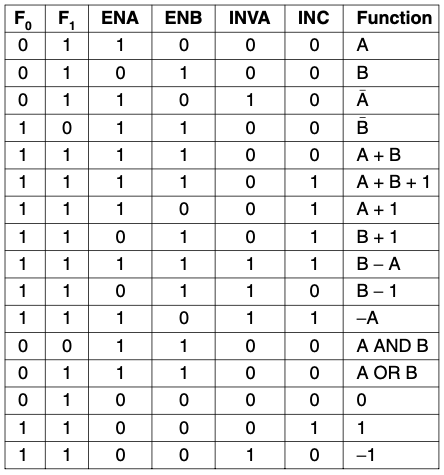
\includegraphics[width=0.7\textwidth]{alu_func.png}
  \caption{Segnali di controllo ALU e relative funzioni}\label{fig:alu_func}
\end{figure}

\begin{myvhdl}{alu.vhd}
 entity alu is
  port (
    --! ALU control
    control       : in  alu_ctrl_type;
    --! ALU operand A
    operand_a     : in  reg_data_type;
    --! ALU operand B
    operand_b     : in  reg_data_type;
    --! ALU result
    sh_result     : out reg_data_type;
    --! Negative flag
    negative_flag : out std_logic;
    --! Zero flag
    zero_flag     : out std_logic
    );
end entity alu;
\end{myvhdl}

\begin{myvhdl}{common\_defs.vhd}
--! Contains common definitions for the processor design.
package common_defs is
  -- Data widths
  --! Processor register data width
  constant reg_data_width      : positive := 32;
  --! MBR register data width
  constant mbr_data_width      : positive := 8;
  --! ALU control width
  constant alu_ctrl_width      : positive := 8;

  [...]

  -- Subtypes
  --! Processor register data
  subtype reg_data_type is std_logic_vector(reg_data_width - 1 downto 0);
  --! MBR register data
  subtype mbr_data_type is std_logic_vector(mbr_data_width - 1 downto 0);
  --! ALU control type
  subtype alu_ctrl_type is std_logic_vector(alu_ctrl_width - 1 downto 0);

  [...]

end package common_defs;
\end{myvhdl}

\subsection{L'Interfaccia con la Memoria}

\section{Le Microistruzioni}

\section{L'Unità di Controllo}

\chapter{Il Livello ISA}

\section{Macchine a Stack}

\chapter{Installazione}

\begin{commandshell}
  apt-get install ghdl
\end{commandshell}

\begin{thebibliography}{2}
  \bibitem{tanenbaum}
  Andrew S. Tanenbaum e Todd Austin.
  \textit{Structured Computer Organization}.
  Pearson, 2013.

  \bibitem{calc}
  Gianni Conte, Antonino Mazzeo, Nicola Mazzocca e Paolo Prinetto.
  \textit{Architettura dei Calcolatori}.
  CittàStudi, 2015.
\end{thebibliography}
\end{document}
